\documentclass[Softwaredesign/Softwaredesign_main.tex]{subfiles}
\begin{document}
\section{CupLight\_IF Software Design}
Til at kontrollere lyset, der skal være under kopperne, skal der bruges en driver. Dette kapitel vil præsentere nogle af de design valg, der er lavet vedrørende lyset under kopperne.
\subsection{CupLight\_IF Software Design ved multiplexing}
Da pointen ved at bruge en RGB-led er, at der kan styres farven af led'en så laves der derfor et modul \textit{rgb\_led}, som har til formål at stå for at håndtere det farve mæssige i en RGB-led. Som sagt kan farven på en RGB-led styres ved at bruge PWM på benene, så derfor skal den kunne styre 3 pwm generatorer i PSoC creator. Tilhørende til dette modul laves en typedef struktur kaldet \textit{color\_t}, der er en definition af hvad farverne indeholder (rød,grøn og blå). Farverne hertil kan også kun have værdier mellem 0 og 255, hvilkes der bør tages hånd om i farvernes setMetoder.
\\Denne metode kan i sig selv styre bare en LED, og bør derfor passende testes for dette. I princippet kan den også styre flere LED'er, men dette er ikke relevant til beerpong bordet, da alle LED'er vil have samme farve.
\\Til kontrol af flere LED'er bruges PSoC's SPI Master komponent, da denne kan bruges til at shifte ting ind i et shift register. Derudover skal der være et digital output pin, der har til formål at latche outputtet og et pin, der har til formål at enable outputtet på 74hc595. Det samlede design for komponenterne, der er anvendt i PsoC'en kan ses på figur \ref{fig:CupLight_PSoC_Design}.
\begin{figure}[H]
    \centering
    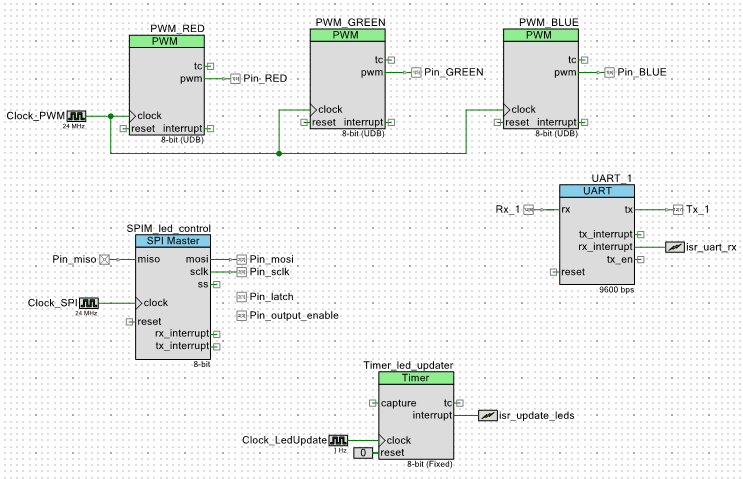
\includegraphics[width=\textwidth]{Softwaredesign/CupLight_IF/graphics/CupLightPSoCDesign.png}
    \caption{PSoC design for CupLight\_IF}
    \label{fig:CupLight_PSoC_Design}
\end{figure}

\subsection{CupLight\_IF Software Design ved ShiftPWM}
Til denne implementering kræves, der noget avanceret bit shifting, i det der skal laves et PWM signal på de forskellige pins. Hertil laves et modul, der hedder ShiftPWM, som har til ansvar at stå for at lave ShiftRegisteret til en PWM generator. Her skal der igen anvendes et SPI Master komponent på PSoC'en for at shifte bits ind i 74HC595, men derudover skal der kun anvendes en timer, der har til formål at interrupte, hver gang der skal ske en opdatering af LED'erne. Det overordnede design kan ses på figur \ref{fig:CupLight_ShiftPWM_PSoC_Design}.

\begin{figure}
    \centering
    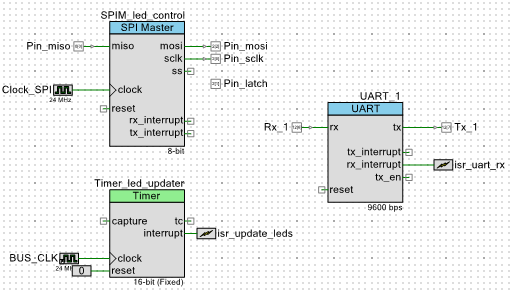
\includegraphics{Softwaredesign/CupLight_IF/graphics/CupLightPSoCDesign_ShiftPWM.png}
    \caption{PSoC desing for CupLight\_IF, der anvender ShiftPWM}
    \label{fig:CupLight_ShiftPWM_PSoC_Design}
\end{figure}

Det ses af figur \ref{fig:CupLight_ShiftPWM_PSoC_Design}, at der er færre komponenter anvendt på PSoC'en (Kun 2, hvis UART til debugging ikke tælles med). Dette er også en klar fordel. Den klare ulempe ved dette design er kompleksiteten af algoritmen, der kan være svær at implementere og få til at virke. En anden klar ulempe er memory usage, idet algoritmen skal bruge en datastruktur, der fylder $ShiftRegData[Resolution \cdot nShiftRegisters]$, hvor resolution er de ønskede steps på PWM signalet og nShiftregisters er antallet 74HC595, der er daisy chained.

\section{Design Diskussion Multiplexing vs. ShiftPMW}
I dete afsnit diskuteres hvorvidt multiplexing eller ShiftPWM anvendes for det pågældende projekt. Starter vi ud med at kigge på \textbf{Multiplexing} så er der nogle klare fordele, så som mindre memory brug og det er nemmere at implementere. Men det har også nogle ulemper, som at der er nogen tuning af timing og at lyset bliver mindre kraftigt, idet lysene er slukket i den periode, hvor de andre opdateres.
\\Ved \textbf{ShiftPWM} skal der højst sandsynligt hentes inspiration ind fra en ekstern kilde, idet det muligvis er for komplekst selv at lave. Det udnytter derimod pins på PSoC'en vanvittigt effektiv idet, der kan styres et nærmest vilkårligt antal LED'er (Der er en upper limit for, hvor mange shiftregisters der kan daisy chaines og fungere). Derudover vil lysene også være kraftigere, hvor tradeoff er det memory, der skal anvendes til at holde styr på, sekvensen af pins, der skal opdateres.
\\Den endelig konklusion er, at det ShiftPWM anvendes, da det bare har for mange fordele i forhold til ulemper i sammenligning med Multiplexing. Der er dog lavet en demo til hver af metoderne, da det var nødvendigt at determinere ud fra en visuel test før en endelig konklusion kunne tages.



\end{document}